\documentclass[1p]{elsarticle_modified}
%\bibliographystyle{elsarticle-num}

%\usepackage[colorlinks]{hyperref}
%\usepackage{abbrmath_seonhwa} %\Abb, \Ascr, \Acal ,\Abf, \Afrak
\usepackage{amsfonts}
\usepackage{amssymb}
\usepackage{amsmath}
\usepackage{amsthm}
\usepackage{scalefnt}
\usepackage{amsbsy}
\usepackage{kotex}
\usepackage{caption}
\usepackage{subfig}
\usepackage{color}
\usepackage{graphicx}
\usepackage{xcolor} %% white, black, red, green, blue, cyan, magenta, yellow
\usepackage{float}
\usepackage{setspace}
\usepackage{hyperref}

\usepackage{tikz}
\usetikzlibrary{arrows}

\usepackage{multirow}
\usepackage{array} % fixed length table
\usepackage{hhline}

%%%%%%%%%%%%%%%%%%%%%
\makeatletter
\renewcommand*\env@matrix[1][\arraystretch]{%
	\edef\arraystretch{#1}%
	\hskip -\arraycolsep
	\let\@ifnextchar\new@ifnextchar
	\array{*\c@MaxMatrixCols c}}
\makeatother %https://tex.stackexchange.com/questions/14071/how-can-i-increase-the-line-spacing-in-a-matrix
%%%%%%%%%%%%%%%

\usepackage[normalem]{ulem}

\newcommand{\msout}[1]{\ifmmode\text{\sout{\ensuremath{#1}}}\else\sout{#1}\fi}
%SOURCE: \msout is \stkout macro in https://tex.stackexchange.com/questions/20609/strikeout-in-math-mode

\newcommand{\cancel}[1]{
	\ifmmode
	{\color{red}\msout{#1}}
	\else
	{\color{red}\sout{#1}}
	\fi
}

\newcommand{\add}[1]{
	{\color{blue}\uwave{#1}}
}

\newcommand{\replace}[2]{
	\ifmmode
	{\color{red}\msout{#1}}{\color{blue}\uwave{#2}}
	\else
	{\color{red}\sout{#1}}{\color{blue}\uwave{#2}}
	\fi
}

\newcommand{\Sol}{\mathcal{S}} %segment
\newcommand{\D}{D} %diagram
\newcommand{\A}{\mathcal{A}} %arc


%%%%%%%%%%%%%%%%%%%%%%%%%%%%%5 test

\def\sl{\operatorname{\textup{SL}}(2,\Cbb)}
\def\psl{\operatorname{\textup{PSL}}(2,\Cbb)}
\def\quan{\mkern 1mu \triangleright \mkern 1mu}

\theoremstyle{definition}
\newtheorem{thm}{Theorem}[section]
\newtheorem{prop}[thm]{Proposition}
\newtheorem{lem}[thm]{Lemma}
\newtheorem{ques}[thm]{Question}
\newtheorem{cor}[thm]{Corollary}
\newtheorem{defn}[thm]{Definition}
\newtheorem{exam}[thm]{Example}
\newtheorem{rmk}[thm]{Remark}
\newtheorem{alg}[thm]{Algorithm}

\newcommand{\I}{\sqrt{-1}}
\begin{document}

%\begin{frontmatter}
%
%\title{Boundary parabolic representations of knots up to 8 crossings}
%
%%% Group authors per affiliation:
%\author{Yunhi Cho} 
%\address{Department of Mathematics, University of Seoul, Seoul, Korea}
%\ead{yhcho@uos.ac.kr}
%
%
%\author{Seonhwa Kim} %\fnref{s_kim}}
%\address{Center for Geometry and Physics, Institute for Basic Science, Pohang, 37673, Korea}
%\ead{ryeona17@ibs.re.kr}
%
%\author{Hyuk Kim}
%\address{Department of Mathematical Sciences, Seoul National University, Seoul 08826, Korea}
%\ead{hyukkim@snu.ac.kr}
%
%\author{Seokbeom Yoon}
%\address{Department of Mathematical Sciences, Seoul National University, Seoul, 08826,  Korea}
%\ead{sbyoon15@snu.ac.kr}
%
%\begin{abstract}
%We find all boundary parabolic representation of knots up to 8 crossings.
%
%\end{abstract}
%\begin{keyword}
%    \MSC[2010] 57M25 
%\end{keyword}
%
%\end{frontmatter}

%\linenumbers
%\tableofcontents
%
\newcommand\colored[1]{\textcolor{white}{\rule[-0.35ex]{0.8em}{1.4ex}}\kern-0.8em\color{red} #1}%
%\newcommand\colored[1]{\textcolor{white}{ #1}\kern-2.17ex	\textcolor{white}{ #1}\kern-1.81ex	\textcolor{white}{ #1}\kern-2.15ex\color{red}#1	}

{\Large $\underline{11a_{272}~(K11a_{272})}$}

\setlength{\tabcolsep}{10pt}
\renewcommand{\arraystretch}{1.6}
\vspace{1cm}\begin{tabular}{m{100pt}>{\centering\arraybackslash}m{274pt}}
\multirow{5}{120pt}{
	\centering
	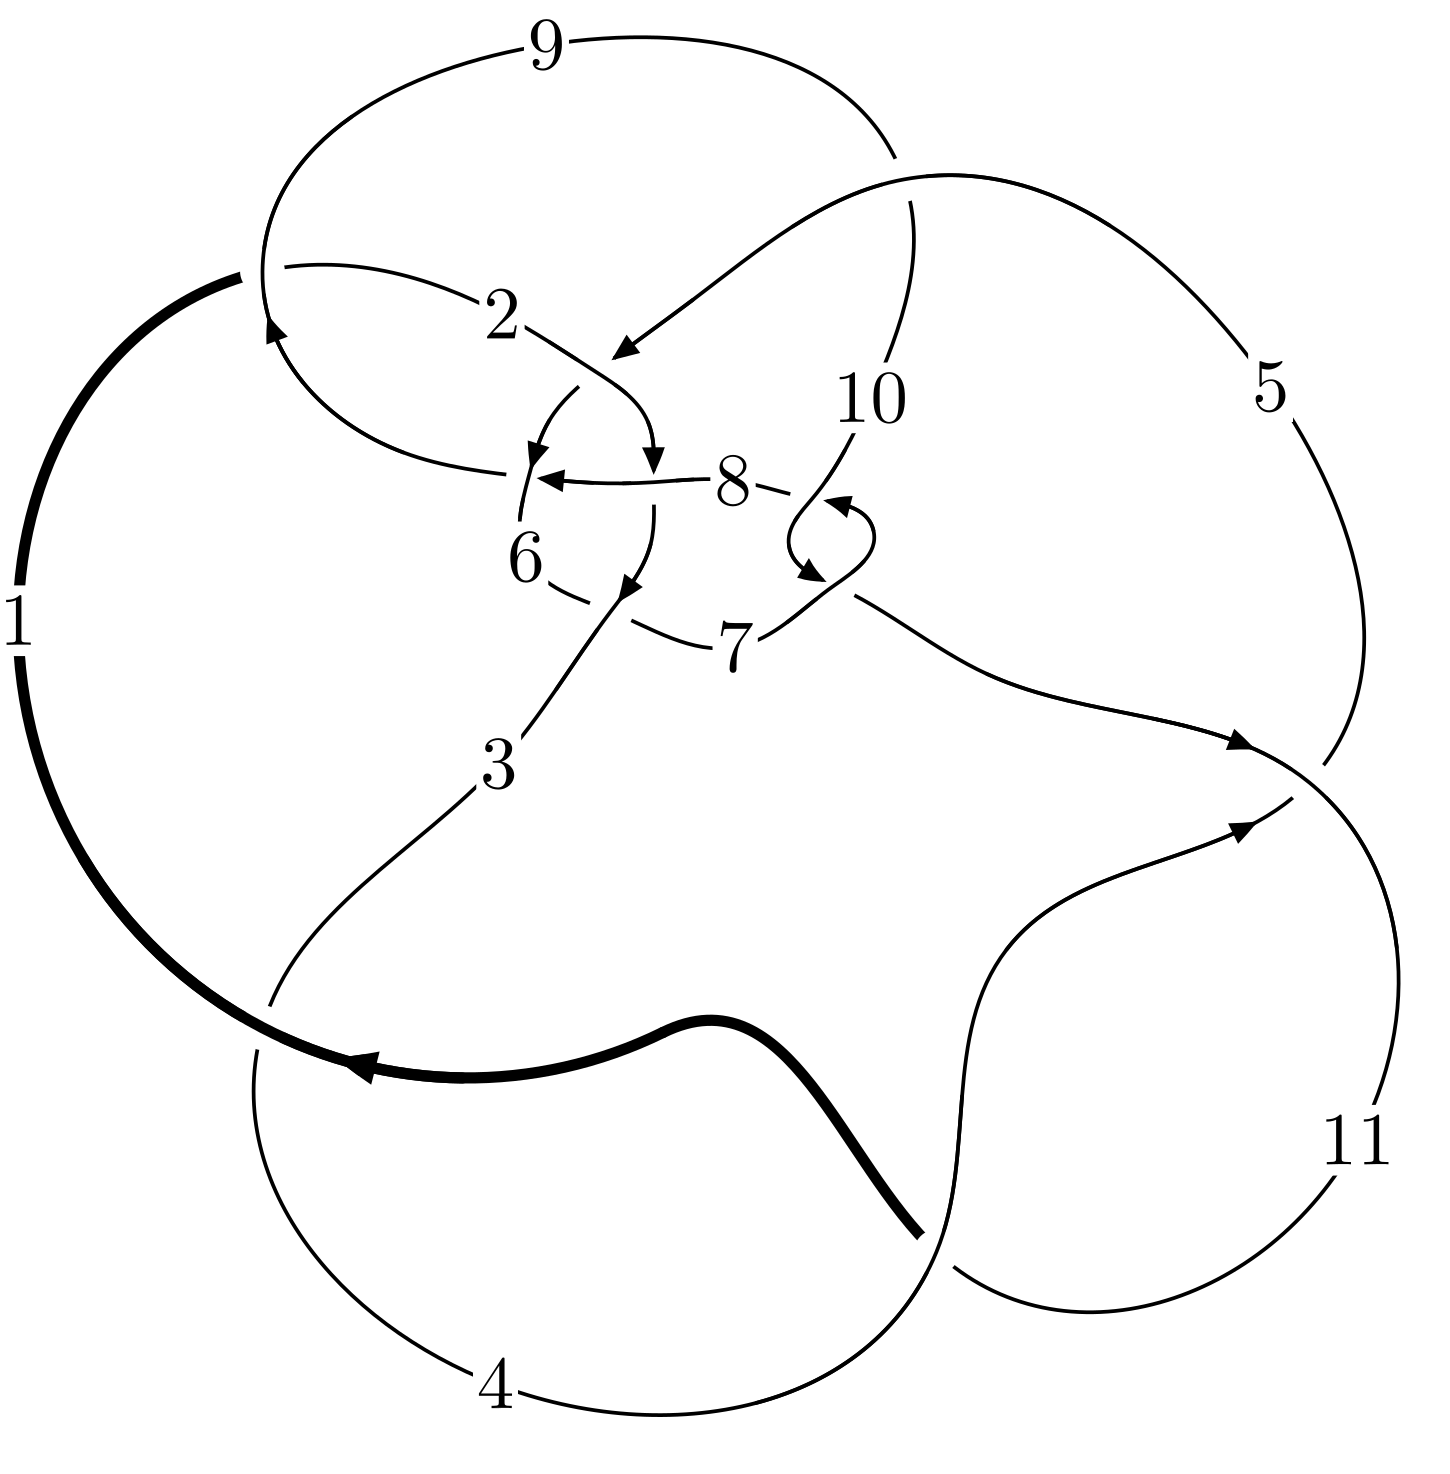
\includegraphics[width=112pt]{../../../GIT/diagram.site/Diagrams/png/521_11a_272.png}\\
\ \ \ A knot diagram\footnotemark}&
\allowdisplaybreaks
\textbf{Linearized knot diagam} \\
\cline{2-2}
 &
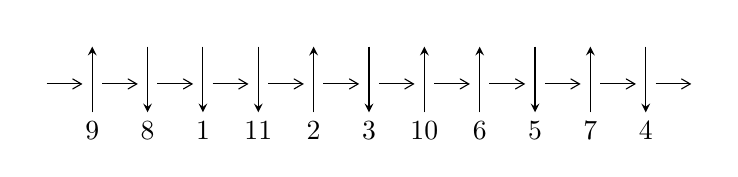
\begin{tikzpicture}[x=20pt, y=17pt]
	% nodes
	\node (C0) at (0, 0) {};
	\node (C1) at (1, 0) {};
	\node (C1U) at (1, +1) {};
	\node (C1D) at (1, -1) {9};

	\node (C2) at (2, 0) {};
	\node (C2U) at (2, +1) {};
	\node (C2D) at (2, -1) {8};

	\node (C3) at (3, 0) {};
	\node (C3U) at (3, +1) {};
	\node (C3D) at (3, -1) {1};

	\node (C4) at (4, 0) {};
	\node (C4U) at (4, +1) {};
	\node (C4D) at (4, -1) {11};

	\node (C5) at (5, 0) {};
	\node (C5U) at (5, +1) {};
	\node (C5D) at (5, -1) {2};

	\node (C6) at (6, 0) {};
	\node (C6U) at (6, +1) {};
	\node (C6D) at (6, -1) {3};

	\node (C7) at (7, 0) {};
	\node (C7U) at (7, +1) {};
	\node (C7D) at (7, -1) {10};

	\node (C8) at (8, 0) {};
	\node (C8U) at (8, +1) {};
	\node (C8D) at (8, -1) {6};

	\node (C9) at (9, 0) {};
	\node (C9U) at (9, +1) {};
	\node (C9D) at (9, -1) {5};

	\node (C10) at (10, 0) {};
	\node (C10U) at (10, +1) {};
	\node (C10D) at (10, -1) {7};

	\node (C11) at (11, 0) {};
	\node (C11U) at (11, +1) {};
	\node (C11D) at (11, -1) {4};
	\node (C12) at (12, 0) {};

	% arrows
	\draw[->,>={angle 60}]
	(C0) edge (C1) (C1) edge (C2) (C2) edge (C3) (C3) edge (C4) (C4) edge (C5) (C5) edge (C6) (C6) edge (C7) (C7) edge (C8) (C8) edge (C9) (C9) edge (C10) (C10) edge (C11) (C11) edge (C12) ;	\draw[->,>=stealth]
	(C1D) edge (C1U) (C2U) edge (C2D) (C3U) edge (C3D) (C4U) edge (C4D) (C5D) edge (C5U) (C6U) edge (C6D) (C7D) edge (C7U) (C8D) edge (C8U) (C9U) edge (C9D) (C10D) edge (C10U) (C11U) edge (C11D) ;
	\end{tikzpicture} \\
\hhline{~~} \\& 
\textbf{Solving Sequence} \\ \cline{2-2} 
 &
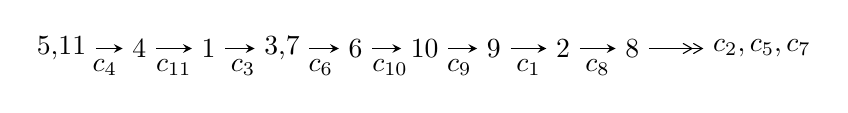
\begin{tikzpicture}[x=25pt, y=7pt]
	% node
	\node (A0) at (-1/8, 0) {5,11};
	\node (A1) at (1, 0) {4};
	\node (A2) at (2, 0) {1};
	\node (A3) at (49/16, 0) {3,7};
	\node (A4) at (33/8, 0) {6};
	\node (A5) at (41/8, 0) {10};
	\node (A6) at (49/8, 0) {9};
	\node (A7) at (57/8, 0) {2};
	\node (A8) at (65/8, 0) {8};
	\node (C1) at (1/2, -1) {$c_{4}$};
	\node (C2) at (3/2, -1) {$c_{11}$};
	\node (C3) at (5/2, -1) {$c_{3}$};
	\node (C4) at (29/8, -1) {$c_{6}$};
	\node (C5) at (37/8, -1) {$c_{10}$};
	\node (C6) at (45/8, -1) {$c_{9}$};
	\node (C7) at (53/8, -1) {$c_{1}$};
	\node (C8) at (61/8, -1) {$c_{8}$};
	\node (A9) at (10, 0) {$c_{2},c_{5},c_{7}$};

	% edge
	\draw[->,>=stealth]	
	(A0) edge (A1) (A1) edge (A2) (A2) edge (A3) (A3) edge (A4) (A4) edge (A5) (A5) edge (A6) (A6) edge (A7) (A7) edge (A8) ;
	\draw[->>,>={angle 60}]	
	(A8) edge (A9);
\end{tikzpicture} \\ 

\end{tabular} \\

\footnotetext{
The image of knot diagram is generated by the software ``\textbf{Draw programme}" developed by Andrew Bartholomew(\url{http://www.layer8.co.uk/maths/draw/index.htm\#Running-draw}), where we modified some parts for our purpose(\url{https://github.com/CATsTAILs/LinksPainter}).
}\phantom \\ \newline 
\centering \textbf{Ideals for irreducible components\footnotemark of $X_{\text{par}}$} 
 
\begin{align*}
I^u_{1}&=\langle 
-3.61113\times10^{167} u^{92}+2.18472\times10^{168} u^{91}+\cdots+6.37635\times10^{168} b+3.55089\times10^{168},\\
\phantom{I^u_{1}}&\phantom{= \langle  }-9.18713\times10^{168} u^{92}+2.85060\times10^{169} u^{91}+\cdots+6.37635\times10^{168} a-2.67247\times10^{170},\\
\phantom{I^u_{1}}&\phantom{= \langle  }u^{93}-3 u^{92}+\cdots+35 u+1\rangle \\
I^u_{2}&=\langle 
- u^{18}-4 u^{17}+\cdots+b+1,\;-3 u^{18}-12 u^{17}+\cdots+a-6,\;u^{19}+4 u^{18}+\cdots+6 u+1\rangle \\
\\
\end{align*}
\raggedright * 2 irreducible components of $\dim_{\mathbb{C}}=0$, with total 112 representations.\\
\footnotetext{All coefficients of polynomials are rational numbers. But the coefficients are sometimes approximated in decimal forms when there is not enough margin.}
\newpage
\renewcommand{\arraystretch}{1}
\centering \section*{I. $I^u_{1}= \langle -3.61\times10^{167} u^{92}+2.18\times10^{168} u^{91}+\cdots+6.38\times10^{168} b+3.55\times10^{168},\;-9.19\times10^{168} u^{92}+2.85\times10^{169} u^{91}+\cdots+6.38\times10^{168} a-2.67\times10^{170},\;u^{93}-3 u^{92}+\cdots+35 u+1 \rangle$}
\flushleft \textbf{(i) Arc colorings}\\
\begin{tabular}{m{7pt} m{180pt} m{7pt} m{180pt} }
\flushright $a_{5}=$&$\begin{pmatrix}1\\0\end{pmatrix}$ \\
\flushright $a_{11}=$&$\begin{pmatrix}0\\u\end{pmatrix}$ \\
\flushright $a_{4}=$&$\begin{pmatrix}1\\- u^2\end{pmatrix}$ \\
\flushright $a_{1}=$&$\begin{pmatrix}- u\\u^3+u\end{pmatrix}$ \\
\flushright $a_{3}=$&$\begin{pmatrix}u^2+1\\- u^4-2 u^2\end{pmatrix}$ \\
\flushright $a_{7}=$&$\begin{pmatrix}1.44081 u^{92}-4.47059 u^{91}+\cdots+218.541 u+41.9122\\0.0566333 u^{92}-0.342629 u^{91}+\cdots-7.62012 u-0.556885\end{pmatrix}$ \\
\flushright $a_{6}=$&$\begin{pmatrix}1.42259 u^{92}-4.52646 u^{91}+\cdots+214.273 u+41.5325\\-0.0227635 u^{92}+0.0219528 u^{91}+\cdots-5.44936 u-0.491557\end{pmatrix}$ \\
\flushright $a_{10}=$&$\begin{pmatrix}1.77836 u^{92}-5.34281 u^{91}+\cdots+274.509 u+50.4757\\-0.0631020 u^{92}+0.374452 u^{91}+\cdots-2.47058 u-0.512941\end{pmatrix}$ \\
\flushright $a_{9}=$&$\begin{pmatrix}1.71526 u^{92}-4.96836 u^{91}+\cdots+272.038 u+49.9627\\-0.0631020 u^{92}+0.374452 u^{91}+\cdots-2.47058 u-0.512941\end{pmatrix}$ \\
\flushright $a_{2}=$&$\begin{pmatrix}-2.58352 u^{92}+7.76269 u^{91}+\cdots-386.533 u-70.1350\\-0.106632 u^{92}+0.379755 u^{91}+\cdots+5.53474 u+0.757562\end{pmatrix}$ \\
\flushright $a_{8}=$&$\begin{pmatrix}3.39815 u^{92}-10.1775 u^{91}+\cdots+545.871 u+102.229\\0.0767390 u^{92}-0.283264 u^{91}+\cdots-7.14975 u-1.07497\end{pmatrix}$\\ \flushright $a_{8}=$&$\begin{pmatrix}3.39815 u^{92}-10.1775 u^{91}+\cdots+545.871 u+102.229\\0.0767390 u^{92}-0.283264 u^{91}+\cdots-7.14975 u-1.07497\end{pmatrix}$\\&\end{tabular}
\flushleft \textbf{(ii) Obstruction class $= -1$}\\~\\
\flushleft \textbf{(iii) Cusp Shapes $= 0.120851 u^{92}-0.494471 u^{91}+\cdots+138.022 u+32.4350$}\\~\\
\newpage\renewcommand{\arraystretch}{1}
\flushleft \textbf{(iv) u-Polynomials at the component}\newline \\
\begin{tabular}{m{50pt}|m{274pt}}
Crossings & \hspace{64pt}u-Polynomials at each crossing \\
\hline $$\begin{aligned}c_{1}\end{aligned}$$&$\begin{aligned}
&u^{93}-4 u^{92}+\cdots-31 u-1
\end{aligned}$\\
\hline $$\begin{aligned}c_{2}\end{aligned}$$&$\begin{aligned}
&u^{93}- u^{92}+\cdots-16 u^2-1
\end{aligned}$\\
\hline $$\begin{aligned}c_{3},c_{4},c_{11}\end{aligned}$$&$\begin{aligned}
&u^{93}+3 u^{92}+\cdots+35 u-1
\end{aligned}$\\
\hline $$\begin{aligned}c_{5}\end{aligned}$$&$\begin{aligned}
&u^{93}-2 u^{92}+\cdots-55 u^2+5
\end{aligned}$\\
\hline $$\begin{aligned}c_{6}\end{aligned}$$&$\begin{aligned}
&u^{93}- u^{92}+\cdots+1077 u-389
\end{aligned}$\\
\hline $$\begin{aligned}c_{7},c_{10}\end{aligned}$$&$\begin{aligned}
&u^{93}-5 u^{92}+\cdots-780 u-145
\end{aligned}$\\
\hline $$\begin{aligned}c_{8}\end{aligned}$$&$\begin{aligned}
&u^{93}+6 u^{92}+\cdots-15 u-1
\end{aligned}$\\
\hline $$\begin{aligned}c_{9}\end{aligned}$$&$\begin{aligned}
&u^{93}+u^{92}+\cdots+200551 u-22691
\end{aligned}$\\
\hline
\end{tabular}\\~\\
\newpage\renewcommand{\arraystretch}{1}
\flushleft \textbf{(v) Riley Polynomials at the component}\newline \\
\begin{tabular}{m{50pt}|m{274pt}}
Crossings & \hspace{64pt}Riley Polynomials at each crossing \\
\hline $$\begin{aligned}c_{1}\end{aligned}$$&$\begin{aligned}
&y^{93}-8 y^{92}+\cdots+187 y-1
\end{aligned}$\\
\hline $$\begin{aligned}c_{2}\end{aligned}$$&$\begin{aligned}
&y^{93}-3 y^{92}+\cdots-32 y-1
\end{aligned}$\\
\hline $$\begin{aligned}c_{3},c_{4},c_{11}\end{aligned}$$&$\begin{aligned}
&y^{93}+89 y^{92}+\cdots+865 y-1
\end{aligned}$\\
\hline $$\begin{aligned}c_{5}\end{aligned}$$&$\begin{aligned}
&y^{93}-2 y^{92}+\cdots+550 y-25
\end{aligned}$\\
\hline $$\begin{aligned}c_{6}\end{aligned}$$&$\begin{aligned}
&y^{93}- y^{92}+\cdots+10281979 y-151321
\end{aligned}$\\
\hline $$\begin{aligned}c_{7},c_{10}\end{aligned}$$&$\begin{aligned}
&y^{93}+47 y^{92}+\cdots-487800 y-21025
\end{aligned}$\\
\hline $$\begin{aligned}c_{8}\end{aligned}$$&$\begin{aligned}
&y^{93}+82 y^{91}+\cdots-11 y-1
\end{aligned}$\\
\hline $$\begin{aligned}c_{9}\end{aligned}$$&$\begin{aligned}
&y^{93}+11 y^{92}+\cdots-8110309523 y-514881481
\end{aligned}$\\
\hline
\end{tabular}\\~\\
\newpage\flushleft \textbf{(vi) Complex Volumes and Cusp Shapes}
$$\begin{array}{c|c|c}  
\text{Solutions to }I^u_{1}& \I (\text{vol} + \sqrt{-1}CS) & \text{Cusp shape}\\
 \hline 
\begin{aligned}
u &= -0.911459 + 0.395130 I \\
a &= -0.060081 - 1.366940 I \\
b &= \phantom{-}0.51305 + 1.76784 I\end{aligned}
 & -2.34640 + 13.18230 I & \phantom{-0.000000 } 0 \\ \hline\begin{aligned}
u &= -0.911459 - 0.395130 I \\
a &= -0.060081 + 1.366940 I \\
b &= \phantom{-}0.51305 - 1.76784 I\end{aligned}
 & -2.34640 - 13.18230 I & \phantom{-0.000000 } 0 \\ \hline\begin{aligned}
u &= \phantom{-}0.246625 + 0.978794 I \\
a &= \phantom{-}0.958092 + 0.139258 I \\
b &= \phantom{-}0.448747 + 0.173387 I\end{aligned}
 & \phantom{-}0.12781 - 2.07574 I & \phantom{-0.000000 } 0 \\ \hline\begin{aligned}
u &= \phantom{-}0.246625 - 0.978794 I \\
a &= \phantom{-}0.958092 - 0.139258 I \\
b &= \phantom{-}0.448747 - 0.173387 I\end{aligned}
 & \phantom{-}0.12781 + 2.07574 I & \phantom{-0.000000 } 0 \\ \hline\begin{aligned}
u &= \phantom{-}0.974658 + 0.386518 I \\
a &= \phantom{-}0.113415 + 1.095790 I \\
b &= \phantom{-}0.60161 - 1.59436 I\end{aligned}
 & -3.52135 - 3.76961 I & \phantom{-0.000000 } 0 \\ \hline\begin{aligned}
u &= \phantom{-}0.974658 - 0.386518 I \\
a &= \phantom{-}0.113415 - 1.095790 I \\
b &= \phantom{-}0.60161 + 1.59436 I\end{aligned}
 & -3.52135 + 3.76961 I & \phantom{-0.000000 } 0 \\ \hline\begin{aligned}
u &= \phantom{-}0.955720 + 0.446072 I \\
a &= -0.055176 - 1.052380 I \\
b &= -0.22885 + 1.73553 I\end{aligned}
 & -3.32185 - 4.23352 I & \phantom{-0.000000 } 0 \\ \hline\begin{aligned}
u &= \phantom{-}0.955720 - 0.446072 I \\
a &= -0.055176 + 1.052380 I \\
b &= -0.22885 - 1.73553 I\end{aligned}
 & -3.32185 + 4.23352 I & \phantom{-0.000000 } 0 \\ \hline\begin{aligned}
u &= -0.756553 + 0.865886 I \\
a &= -0.974997 + 0.306547 I \\
b &= -0.243449 - 1.167070 I\end{aligned}
 & -0.98495 - 7.52546 I & \phantom{-0.000000 } 0 \\ \hline\begin{aligned}
u &= -0.756553 - 0.865886 I \\
a &= -0.974997 - 0.306547 I \\
b &= -0.243449 + 1.167070 I\end{aligned}
 & -0.98495 + 7.52546 I & \phantom{-0.000000 } 0\\
 \hline 
 \end{array}$$\newpage$$\begin{array}{c|c|c}  
\text{Solutions to }I^u_{1}& \I (\text{vol} + \sqrt{-1}CS) & \text{Cusp shape}\\
 \hline 
\begin{aligned}
u &= \phantom{-}0.732299 + 0.909796 I \\
a &= \phantom{-}0.707676 + 0.298865 I \\
b &= \phantom{-}0.879779 - 0.946817 I\end{aligned}
 & -2.03674 - 1.66542 I & \phantom{-0.000000 } 0 \\ \hline\begin{aligned}
u &= \phantom{-}0.732299 - 0.909796 I \\
a &= \phantom{-}0.707676 - 0.298865 I \\
b &= \phantom{-}0.879779 + 0.946817 I\end{aligned}
 & -2.03674 + 1.66542 I & \phantom{-0.000000 } 0 \\ \hline\begin{aligned}
u &= \phantom{-}0.602610 + 0.551898 I \\
a &= \phantom{-}0.57808 + 1.50406 I \\
b &= \phantom{-}0.617201 - 1.013870 I\end{aligned}
 & -1.66403 - 4.99482 I & \phantom{-0.000000 -}0. + 12.04743 I \\ \hline\begin{aligned}
u &= \phantom{-}0.602610 - 0.551898 I \\
a &= \phantom{-}0.57808 - 1.50406 I \\
b &= \phantom{-}0.617201 + 1.013870 I\end{aligned}
 & -1.66403 + 4.99482 I & \phantom{-0.000000 } 0. - 12.04743 I \\ \hline\begin{aligned}
u &= \phantom{-}0.210852 + 1.187670 I \\
a &= -0.543462 - 0.727634 I \\
b &= -0.24590 + 1.78211 I\end{aligned}
 & \phantom{-}0.59025 - 5.59173 I & \phantom{-0.000000 } 0 \\ \hline\begin{aligned}
u &= \phantom{-}0.210852 - 1.187670 I \\
a &= -0.543462 + 0.727634 I \\
b &= -0.24590 - 1.78211 I\end{aligned}
 & \phantom{-}0.59025 + 5.59173 I & \phantom{-0.000000 } 0 \\ \hline\begin{aligned}
u &= -0.042552 + 1.208860 I \\
a &= \phantom{-}1.181090 + 0.101333 I \\
b &= \phantom{-}1.82870 + 0.41508 I\end{aligned}
 & -1.60314 - 3.04863 I & \phantom{-0.000000 } 0 \\ \hline\begin{aligned}
u &= -0.042552 - 1.208860 I \\
a &= \phantom{-}1.181090 - 0.101333 I \\
b &= \phantom{-}1.82870 - 0.41508 I\end{aligned}
 & -1.60314 + 3.04863 I & \phantom{-0.000000 } 0 \\ \hline\begin{aligned}
u &= \phantom{-}0.738015 + 0.267719 I \\
a &= -0.644949 - 1.095980 I \\
b &= \phantom{-}0.58532 + 1.33188 I\end{aligned}
 & -2.67687 + 0.69646 I & -9.23370 + 0.62043 I \\ \hline\begin{aligned}
u &= \phantom{-}0.738015 - 0.267719 I \\
a &= -0.644949 + 1.095980 I \\
b &= \phantom{-}0.58532 - 1.33188 I\end{aligned}
 & -2.67687 - 0.69646 I & -9.23370 - 0.62043 I\\
 \hline 
 \end{array}$$\newpage$$\begin{array}{c|c|c}  
\text{Solutions to }I^u_{1}& \I (\text{vol} + \sqrt{-1}CS) & \text{Cusp shape}\\
 \hline 
\begin{aligned}
u &= \phantom{-}0.777826 + 0.016678 I \\
a &= \phantom{-}0.62554 - 1.27383 I \\
b &= \phantom{-}0.198182 + 1.154930 I\end{aligned}
 & -2.91425 - 1.94861 I & -10.28563 + 0.40390 I \\ \hline\begin{aligned}
u &= \phantom{-}0.777826 - 0.016678 I \\
a &= \phantom{-}0.62554 + 1.27383 I \\
b &= \phantom{-}0.198182 - 1.154930 I\end{aligned}
 & -2.91425 + 1.94861 I & -10.28563 - 0.40390 I \\ \hline\begin{aligned}
u &= \phantom{-}0.288392 + 0.707750 I \\
a &= \phantom{-}0.768676 + 0.217271 I \\
b &= \phantom{-}0.005605 + 0.312661 I\end{aligned}
 & \phantom{-}0.13872 - 2.01683 I & \phantom{-}0.67333 + 3.98715 I \\ \hline\begin{aligned}
u &= \phantom{-}0.288392 - 0.707750 I \\
a &= \phantom{-}0.768676 - 0.217271 I \\
b &= \phantom{-}0.005605 - 0.312661 I\end{aligned}
 & \phantom{-}0.13872 + 2.01683 I & \phantom{-}0.67333 - 3.98715 I \\ \hline\begin{aligned}
u &= -0.654822 + 0.391719 I \\
a &= -1.263680 - 0.402248 I \\
b &= \phantom{-}0.260205 - 0.435804 I\end{aligned}
 & \phantom{-}0.67894 + 7.53424 I & -0.24390 - 7.52483 I \\ \hline\begin{aligned}
u &= -0.654822 - 0.391719 I \\
a &= -1.263680 + 0.402248 I \\
b &= \phantom{-}0.260205 + 0.435804 I\end{aligned}
 & \phantom{-}0.67894 - 7.53424 I & -0.24390 + 7.52483 I \\ \hline\begin{aligned}
u &= -0.591766 + 0.464752 I \\
a &= -0.154401 - 0.822190 I \\
b &= \phantom{-}0.82840 + 1.15264 I\end{aligned}
 & \phantom{-}1.00153 - 3.54334 I & \phantom{-}1.58809 + 0.30458 I \\ \hline\begin{aligned}
u &= -0.591766 - 0.464752 I \\
a &= -0.154401 + 0.822190 I \\
b &= \phantom{-}0.82840 - 1.15264 I\end{aligned}
 & \phantom{-}1.00153 + 3.54334 I & \phantom{-}1.58809 - 0.30458 I \\ \hline\begin{aligned}
u &= \phantom{-}0.812390 + 0.967240 I \\
a &= -0.587684 - 0.393263 I \\
b &= -0.394533 + 1.276390 I\end{aligned}
 & -1.92498 - 2.34475 I & \phantom{-0.000000 } 0 \\ \hline\begin{aligned}
u &= \phantom{-}0.812390 - 0.967240 I \\
a &= -0.587684 + 0.393263 I \\
b &= -0.394533 - 1.276390 I\end{aligned}
 & -1.92498 + 2.34475 I & \phantom{-0.000000 } 0\\
 \hline 
 \end{array}$$\newpage$$\begin{array}{c|c|c}  
\text{Solutions to }I^u_{1}& \I (\text{vol} + \sqrt{-1}CS) & \text{Cusp shape}\\
 \hline 
\begin{aligned}
u &= -0.672569 + 0.279083 I \\
a &= \phantom{-}0.06726 + 1.89775 I \\
b &= -0.49534 - 1.65370 I\end{aligned}
 & -1.19275 + 5.34921 I & \phantom{-}0.55034 - 10.82397 I \\ \hline\begin{aligned}
u &= -0.672569 - 0.279083 I \\
a &= \phantom{-}0.06726 - 1.89775 I \\
b &= -0.49534 + 1.65370 I\end{aligned}
 & -1.19275 - 5.34921 I & \phantom{-}0.55034 + 10.82397 I \\ \hline\begin{aligned}
u &= \phantom{-}0.003533 + 1.274680 I \\
a &= \phantom{-}0.525082 + 0.174725 I \\
b &= \phantom{-}0.54755 - 2.88462 I\end{aligned}
 & \phantom{-}2.75039 + 4.22339 I & \phantom{-0.000000 } 0 \\ \hline\begin{aligned}
u &= \phantom{-}0.003533 - 1.274680 I \\
a &= \phantom{-}0.525082 - 0.174725 I \\
b &= \phantom{-}0.54755 + 2.88462 I\end{aligned}
 & \phantom{-}2.75039 - 4.22339 I & \phantom{-0.000000 } 0 \\ \hline\begin{aligned}
u &= -0.117069 + 1.283880 I \\
a &= -1.315870 + 0.095206 I \\
b &= -1.012990 - 0.406576 I\end{aligned}
 & -1.28790 + 5.38199 I & \phantom{-0.000000 } 0 \\ \hline\begin{aligned}
u &= -0.117069 - 1.283880 I \\
a &= -1.315870 - 0.095206 I \\
b &= -1.012990 + 0.406576 I\end{aligned}
 & -1.28790 - 5.38199 I & \phantom{-0.000000 } 0 \\ \hline\begin{aligned}
u &= -0.176650 + 1.277580 I \\
a &= \phantom{-}0.799827 - 0.504979 I \\
b &= \phantom{-}0.09805 + 1.48760 I\end{aligned}
 & -0.818431 - 0.586473 I & \phantom{-0.000000 } 0 \\ \hline\begin{aligned}
u &= -0.176650 - 1.277580 I \\
a &= \phantom{-}0.799827 + 0.504979 I \\
b &= \phantom{-}0.09805 - 1.48760 I\end{aligned}
 & -0.818431 + 0.586473 I & \phantom{-0.000000 } 0 \\ \hline\begin{aligned}
u &= \phantom{-}0.004246 + 1.329120 I \\
a &= -0.858955 + 0.481977 I \\
b &= -1.18895 - 1.40669 I\end{aligned}
 & \phantom{-}3.86557 + 1.99478 I & \phantom{-0.000000 } 0 \\ \hline\begin{aligned}
u &= \phantom{-}0.004246 - 1.329120 I \\
a &= -0.858955 - 0.481977 I \\
b &= -1.18895 + 1.40669 I\end{aligned}
 & \phantom{-}3.86557 - 1.99478 I & \phantom{-0.000000 } 0\\
 \hline 
 \end{array}$$\newpage$$\begin{array}{c|c|c}  
\text{Solutions to }I^u_{1}& \I (\text{vol} + \sqrt{-1}CS) & \text{Cusp shape}\\
 \hline 
\begin{aligned}
u &= -0.305242 + 1.326130 I \\
a &= -0.472815 + 0.658481 I \\
b &= -1.51214 - 1.46798 I\end{aligned}
 & \phantom{-}5.23834 + 5.65499 I & \phantom{-0.000000 } 0 \\ \hline\begin{aligned}
u &= -0.305242 - 1.326130 I \\
a &= -0.472815 - 0.658481 I \\
b &= -1.51214 + 1.46798 I\end{aligned}
 & \phantom{-}5.23834 - 5.65499 I & \phantom{-0.000000 } 0 \\ \hline\begin{aligned}
u &= \phantom{-}0.535771 + 0.331980 I \\
a &= \phantom{-}0.561496 - 0.224728 I \\
b &= \phantom{-}0.275495 + 0.063895 I\end{aligned}
 & -1.05560 - 1.04516 I & -5.24999 + 4.73518 I \\ \hline\begin{aligned}
u &= \phantom{-}0.535771 - 0.331980 I \\
a &= \phantom{-}0.561496 + 0.224728 I \\
b &= \phantom{-}0.275495 - 0.063895 I\end{aligned}
 & -1.05560 + 1.04516 I & -5.24999 - 4.73518 I \\ \hline\begin{aligned}
u &= -0.135847 + 1.378470 I \\
a &= \phantom{-}0.378488 + 0.952853 I \\
b &= -0.626385 - 0.559687 I\end{aligned}
 & \phantom{-}7.46821 + 1.40401 I & \phantom{-0.000000 } 0 \\ \hline\begin{aligned}
u &= -0.135847 - 1.378470 I \\
a &= \phantom{-}0.378488 - 0.952853 I \\
b &= -0.626385 + 0.559687 I\end{aligned}
 & \phantom{-}7.46821 - 1.40401 I & \phantom{-0.000000 } 0 \\ \hline\begin{aligned}
u &= \phantom{-}0.275110 + 1.366140 I \\
a &= -0.482588 - 0.137919 I \\
b &= -0.26114 + 1.75093 I\end{aligned}
 & \phantom{-}2.40844 - 2.97328 I & \phantom{-0.000000 } 0 \\ \hline\begin{aligned}
u &= \phantom{-}0.275110 - 1.366140 I \\
a &= -0.482588 + 0.137919 I \\
b &= -0.26114 - 1.75093 I\end{aligned}
 & \phantom{-}2.40844 + 2.97328 I & \phantom{-0.000000 } 0 \\ \hline\begin{aligned}
u &= -0.172915 + 1.402530 I \\
a &= \phantom{-}0.563359 + 0.548099 I \\
b &= -0.151156 + 0.172009 I\end{aligned}
 & \phantom{-}5.61748 - 0.19647 I & \phantom{-0.000000 } 0 \\ \hline\begin{aligned}
u &= -0.172915 - 1.402530 I \\
a &= \phantom{-}0.563359 - 0.548099 I \\
b &= -0.151156 - 0.172009 I\end{aligned}
 & \phantom{-}5.61748 + 0.19647 I & \phantom{-0.000000 } 0\\
 \hline 
 \end{array}$$\newpage$$\begin{array}{c|c|c}  
\text{Solutions to }I^u_{1}& \I (\text{vol} + \sqrt{-1}CS) & \text{Cusp shape}\\
 \hline 
\begin{aligned}
u &= \phantom{-}0.07853 + 1.41526 I \\
a &= -0.385092 + 0.973133 I \\
b &= -0.164397 - 0.529226 I\end{aligned}
 & \phantom{-}7.62011 - 0.60893 I & \phantom{-0.000000 } 0 \\ \hline\begin{aligned}
u &= \phantom{-}0.07853 - 1.41526 I \\
a &= -0.385092 - 0.973133 I \\
b &= -0.164397 + 0.529226 I\end{aligned}
 & \phantom{-}7.62011 + 0.60893 I & \phantom{-0.000000 } 0 \\ \hline\begin{aligned}
u &= -0.576840 + 0.056978 I \\
a &= \phantom{-}1.01392 + 1.04721 I \\
b &= -0.478791 - 0.978508 I\end{aligned}
 & \phantom{-}0.93991 + 2.24276 I & \phantom{-}2.13382 - 6.20149 I \\ \hline\begin{aligned}
u &= -0.576840 - 0.056978 I \\
a &= \phantom{-}1.01392 - 1.04721 I \\
b &= -0.478791 + 0.978508 I\end{aligned}
 & \phantom{-}0.93991 - 2.24276 I & \phantom{-}2.13382 + 6.20149 I \\ \hline\begin{aligned}
u &= -0.16657 + 1.41522 I \\
a &= -0.737844 + 0.359479 I \\
b &= \phantom{-}0.05293 - 2.26413 I\end{aligned}
 & \phantom{-}0.95617 + 6.95484 I & \phantom{-0.000000 } 0 \\ \hline\begin{aligned}
u &= -0.16657 - 1.41522 I \\
a &= -0.737844 - 0.359479 I \\
b &= \phantom{-}0.05293 + 2.26413 I\end{aligned}
 & \phantom{-}0.95617 - 6.95484 I & \phantom{-0.000000 } 0 \\ \hline\begin{aligned}
u &= -0.26162 + 1.41387 I \\
a &= -0.829533 + 0.679950 I \\
b &= -1.27505 - 1.88111 I\end{aligned}
 & \phantom{-}4.22352 + 8.75550 I & \phantom{-0.000000 } 0 \\ \hline\begin{aligned}
u &= -0.26162 - 1.41387 I \\
a &= -0.829533 - 0.679950 I \\
b &= -1.27505 + 1.88111 I\end{aligned}
 & \phantom{-}4.22352 - 8.75550 I & \phantom{-0.000000 } 0 \\ \hline\begin{aligned}
u &= \phantom{-}0.17440 + 1.45659 I \\
a &= -0.717413 - 0.360056 I \\
b &= -1.90212 + 1.94824 I\end{aligned}
 & \phantom{-}5.89949 - 6.94617 I & \phantom{-0.000000 } 0 \\ \hline\begin{aligned}
u &= \phantom{-}0.17440 - 1.45659 I \\
a &= -0.717413 + 0.360056 I \\
b &= -1.90212 - 1.94824 I\end{aligned}
 & \phantom{-}5.89949 + 6.94617 I & \phantom{-0.000000 } 0\\
 \hline 
 \end{array}$$\newpage$$\begin{array}{c|c|c}  
\text{Solutions to }I^u_{1}& \I (\text{vol} + \sqrt{-1}CS) & \text{Cusp shape}\\
 \hline 
\begin{aligned}
u &= -0.527457 + 0.063186 I \\
a &= -0.07687 - 2.62551 I \\
b &= -0.357457 + 1.182460 I\end{aligned}
 & -4.97774 - 3.20790 I & -8.72666 + 3.61708 I \\ \hline\begin{aligned}
u &= -0.527457 - 0.063186 I \\
a &= -0.07687 + 2.62551 I \\
b &= -0.357457 - 1.182460 I\end{aligned}
 & -4.97774 + 3.20790 I & -8.72666 - 3.61708 I \\ \hline\begin{aligned}
u &= -0.24734 + 1.45630 I \\
a &= -0.397332 - 0.787003 I \\
b &= \phantom{-}0.343876 + 0.308196 I\end{aligned}
 & \phantom{-}6.62651 + 10.84470 I & \phantom{-0.000000 } 0 \\ \hline\begin{aligned}
u &= -0.24734 - 1.45630 I \\
a &= -0.397332 + 0.787003 I \\
b &= \phantom{-}0.343876 - 0.308196 I\end{aligned}
 & \phantom{-}6.62651 - 10.84470 I & \phantom{-0.000000 } 0 \\ \hline\begin{aligned}
u &= -0.005024 + 0.519936 I \\
a &= \phantom{-}1.53006 + 0.63638 I \\
b &= -0.128808 + 0.625732 I\end{aligned}
 & \phantom{-}0.19375 - 2.00732 I & \phantom{-}1.90291 + 4.08224 I \\ \hline\begin{aligned}
u &= -0.005024 - 0.519936 I \\
a &= \phantom{-}1.53006 - 0.63638 I \\
b &= -0.128808 - 0.625732 I\end{aligned}
 & \phantom{-}0.19375 + 2.00732 I & \phantom{-}1.90291 - 4.08224 I \\ \hline\begin{aligned}
u &= \phantom{-}0.14435 + 1.47435 I \\
a &= \phantom{-}0.051712 + 0.613325 I \\
b &= -0.177691 - 0.333417 I\end{aligned}
 & \phantom{-}6.55607 - 3.56363 I & \phantom{-0.000000 } 0 \\ \hline\begin{aligned}
u &= \phantom{-}0.14435 - 1.47435 I \\
a &= \phantom{-}0.051712 - 0.613325 I \\
b &= -0.177691 + 0.333417 I\end{aligned}
 & \phantom{-}6.55607 + 3.56363 I & \phantom{-0.000000 } 0 \\ \hline\begin{aligned}
u &= \phantom{-}0.21979 + 1.46839 I \\
a &= \phantom{-}0.370817 - 0.468364 I \\
b &= \phantom{-}0.022326 + 0.589901 I\end{aligned}
 & \phantom{-}4.94375 - 3.83324 I & \phantom{-0.000000 } 0 \\ \hline\begin{aligned}
u &= \phantom{-}0.21979 - 1.46839 I \\
a &= \phantom{-}0.370817 + 0.468364 I \\
b &= \phantom{-}0.022326 - 0.589901 I\end{aligned}
 & \phantom{-}4.94375 + 3.83324 I & \phantom{-0.000000 } 0\\
 \hline 
 \end{array}$$\newpage$$\begin{array}{c|c|c}  
\text{Solutions to }I^u_{1}& \I (\text{vol} + \sqrt{-1}CS) & \text{Cusp shape}\\
 \hline 
\begin{aligned}
u &= -0.19636 + 1.47715 I \\
a &= \phantom{-}0.575084 - 0.439374 I \\
b &= \phantom{-}1.51693 + 1.22032 I\end{aligned}
 & \phantom{-}7.35184 - 0.66069 I & \phantom{-0.000000 } 0 \\ \hline\begin{aligned}
u &= -0.19636 - 1.47715 I \\
a &= \phantom{-}0.575084 + 0.439374 I \\
b &= \phantom{-}1.51693 - 1.22032 I\end{aligned}
 & \phantom{-}7.35184 + 0.66069 I & \phantom{-0.000000 } 0 \\ \hline\begin{aligned}
u &= -0.445879 + 0.223933 I \\
a &= -0.72430 + 2.47527 I \\
b &= \phantom{-}0.63559 - 1.52906 I\end{aligned}
 & -4.38663 + 4.68917 I & -11.13071 - 7.83950 I \\ \hline\begin{aligned}
u &= -0.445879 - 0.223933 I \\
a &= -0.72430 - 2.47527 I \\
b &= \phantom{-}0.63559 + 1.52906 I\end{aligned}
 & -4.38663 - 4.68917 I & -11.13071 + 7.83950 I \\ \hline\begin{aligned}
u &= \phantom{-}0.317173 + 0.374066 I \\
a &= -0.92898 - 1.56886 I \\
b &= -0.69662 + 2.12690 I\end{aligned}
 & -0.13387 - 4.83140 I & -1.38014 + 12.10335 I \\ \hline\begin{aligned}
u &= \phantom{-}0.317173 - 0.374066 I \\
a &= -0.92898 + 1.56886 I \\
b &= -0.69662 - 2.12690 I\end{aligned}
 & -0.13387 + 4.83140 I & -1.38014 - 12.10335 I \\ \hline\begin{aligned}
u &= \phantom{-}0.23285 + 1.49755 I \\
a &= \phantom{-}0.745388 + 0.647957 I \\
b &= \phantom{-}0.86766 - 1.24614 I\end{aligned}
 & \phantom{-}4.93482 - 8.13681 I & \phantom{-0.000000 } 0 \\ \hline\begin{aligned}
u &= \phantom{-}0.23285 - 1.49755 I \\
a &= \phantom{-}0.745388 - 0.647957 I \\
b &= \phantom{-}0.86766 + 1.24614 I\end{aligned}
 & \phantom{-}4.93482 + 8.13681 I & \phantom{-0.000000 } 0 \\ \hline\begin{aligned}
u &= \phantom{-}0.36704 + 1.48082 I \\
a &= \phantom{-}0.728699 + 0.535940 I \\
b &= \phantom{-}1.35721 - 1.37957 I\end{aligned}
 & \phantom{-}2.42961 - 8.56668 I & \phantom{-0.000000 } 0 \\ \hline\begin{aligned}
u &= \phantom{-}0.36704 - 1.48082 I \\
a &= \phantom{-}0.728699 - 0.535940 I \\
b &= \phantom{-}1.35721 + 1.37957 I\end{aligned}
 & \phantom{-}2.42961 + 8.56668 I & \phantom{-0.000000 } 0\\
 \hline 
 \end{array}$$\newpage$$\begin{array}{c|c|c}  
\text{Solutions to }I^u_{1}& \I (\text{vol} + \sqrt{-1}CS) & \text{Cusp shape}\\
 \hline 
\begin{aligned}
u &= -0.34922 + 1.49380 I \\
a &= \phantom{-}0.709563 - 0.650111 I \\
b &= \phantom{-}1.26940 + 1.85557 I\end{aligned}
 & \phantom{-}3.7167 + 17.7393 I & \phantom{-0.000000 } 0 \\ \hline\begin{aligned}
u &= -0.34922 - 1.49380 I \\
a &= \phantom{-}0.709563 + 0.650111 I \\
b &= \phantom{-}1.26940 - 1.85557 I\end{aligned}
 & \phantom{-}3.7167 - 17.7393 I & \phantom{-0.000000 } 0 \\ \hline\begin{aligned}
u &= \phantom{-}0.35894 + 1.51768 I \\
a &= -0.594952 - 0.533137 I \\
b &= -1.05454 + 1.85472 I\end{aligned}
 & \phantom{-}2.98943 - 8.99089 I & \phantom{-0.000000 } 0 \\ \hline\begin{aligned}
u &= \phantom{-}0.35894 - 1.51768 I \\
a &= -0.594952 + 0.533137 I \\
b &= -1.05454 - 1.85472 I\end{aligned}
 & \phantom{-}2.98943 + 8.99089 I & \phantom{-0.000000 } 0 \\ \hline\begin{aligned}
u &= \phantom{-}0.10285 + 1.58207 I \\
a &= \phantom{-}0.322796 - 0.166607 I \\
b &= -0.611667 + 0.333370 I\end{aligned}
 & \phantom{-}7.99033 - 3.67115 I & \phantom{-0.000000 } 0 \\ \hline\begin{aligned}
u &= \phantom{-}0.10285 - 1.58207 I \\
a &= \phantom{-}0.322796 + 0.166607 I \\
b &= -0.611667 - 0.333370 I\end{aligned}
 & \phantom{-}7.99033 + 3.67115 I & \phantom{-0.000000 } 0 \\ \hline\begin{aligned}
u &= -0.100806 + 0.397094 I \\
a &= \phantom{-}2.20139 + 0.48685 I \\
b &= -0.210768 + 0.748546 I\end{aligned}
 & \phantom{-}0.18872 - 2.00916 I & \phantom{-}2.24464 + 3.56470 I \\ \hline\begin{aligned}
u &= -0.100806 - 0.397094 I \\
a &= \phantom{-}2.20139 - 0.48685 I \\
b &= -0.210768 - 0.748546 I\end{aligned}
 & \phantom{-}0.18872 + 2.00916 I & \phantom{-}2.24464 - 3.56470 I \\ \hline\begin{aligned}
u &= -0.186714 + 0.346826 I \\
a &= \phantom{-}1.35275 + 1.99552 I \\
b &= -0.398511 + 0.161176 I\end{aligned}
 & \phantom{-}2.29833 - 0.12628 I & \phantom{-}10.47295 - 1.82234 I \\ \hline\begin{aligned}
u &= -0.186714 - 0.346826 I \\
a &= \phantom{-}1.35275 - 1.99552 I \\
b &= -0.398511 - 0.161176 I\end{aligned}
 & \phantom{-}2.29833 + 0.12628 I & \phantom{-}10.47295 + 1.82234 I\\
 \hline 
 \end{array}$$\newpage$$\begin{array}{c|c|c}  
\text{Solutions to }I^u_{1}& \I (\text{vol} + \sqrt{-1}CS) & \text{Cusp shape}\\
 \hline 
\begin{aligned}
u &= -0.03589 + 1.65255 I \\
a &= -0.401052 - 0.252951 I \\
b &= -0.266809 + 0.186901 I\end{aligned}
 & \phantom{-}8.28168 - 4.75781 I & \phantom{-0.000000 } 0 \\ \hline\begin{aligned}
u &= -0.03589 - 1.65255 I \\
a &= -0.401052 + 0.252951 I \\
b &= -0.266809 - 0.186901 I\end{aligned}
 & \phantom{-}8.28168 + 4.75781 I & \phantom{-0.000000 } 0 \\ \hline\begin{aligned}
u &= -0.0336230\phantom{ +0.000000I} \\
a &= \phantom{-}35.5555\phantom{ +0.000000I} \\
b &= -0.339499\phantom{ +0.000000I}\end{aligned}
 & \phantom{-}2.39628\phantom{ +0.000000I} & \phantom{-}28.3130\phantom{ +0.000000I}\\
 \hline 
 \end{array}$$\newpage\newpage\renewcommand{\arraystretch}{1}
\centering \section*{II. $I^u_{2}= \langle - u^{18}-4 u^{17}+\cdots+b+1,\;-3 u^{18}-12 u^{17}+\cdots+a-6,\;u^{19}+4 u^{18}+\cdots+6 u+1 \rangle$}
\flushleft \textbf{(i) Arc colorings}\\
\begin{tabular}{m{7pt} m{180pt} m{7pt} m{180pt} }
\flushright $a_{5}=$&$\begin{pmatrix}1\\0\end{pmatrix}$ \\
\flushright $a_{11}=$&$\begin{pmatrix}0\\u\end{pmatrix}$ \\
\flushright $a_{4}=$&$\begin{pmatrix}1\\- u^2\end{pmatrix}$ \\
\flushright $a_{1}=$&$\begin{pmatrix}- u\\u^3+u\end{pmatrix}$ \\
\flushright $a_{3}=$&$\begin{pmatrix}u^2+1\\- u^4-2 u^2\end{pmatrix}$ \\
\flushright $a_{7}=$&$\begin{pmatrix}3 u^{18}+12 u^{17}+\cdots+15 u+6\\u^{18}+4 u^{17}+\cdots-3 u-1\end{pmatrix}$ \\
\flushright $a_{6}=$&$\begin{pmatrix}3 u^{18}+12 u^{17}+\cdots+13 u+6\\- u^6-2 u^5-5 u^4-6 u^3-6 u^2-4 u-1\end{pmatrix}$ \\
\flushright $a_{10}=$&$\begin{pmatrix}u^{18}+4 u^{17}+\cdots+8 u+6\\2 u^{17}+7 u^{16}+\cdots+8 u+1\end{pmatrix}$ \\
\flushright $a_{9}=$&$\begin{pmatrix}u^{18}+6 u^{17}+\cdots+16 u+7\\2 u^{17}+7 u^{16}+\cdots+8 u+1\end{pmatrix}$ \\
\flushright $a_{2}=$&$\begin{pmatrix}-3 u^{18}-12 u^{17}+\cdots-30 u-11\\u^3+u^2+2 u+1\end{pmatrix}$ \\
\flushright $a_{8}=$&$\begin{pmatrix}u^{18}+3 u^{17}+\cdots+21 u+14\\2 u^{17}+8 u^{16}+\cdots+13 u^2+5 u\end{pmatrix}$\\ \flushright $a_{8}=$&$\begin{pmatrix}u^{18}+3 u^{17}+\cdots+21 u+14\\2 u^{17}+8 u^{16}+\cdots+13 u^2+5 u\end{pmatrix}$\\&\end{tabular}
\flushleft \textbf{(ii) Obstruction class $= 1$}\\~\\
\flushleft \textbf{(iii) Cusp Shapes $= -6 u^{18}-28 u^{17}-127 u^{16}-363 u^{15}-940 u^{14}-1903 u^{13}-3460 u^{12}-5244 u^{11}-7119 u^{10}-8212 u^9-8436 u^8-7329 u^7-5610 u^6-3541 u^5-1966 u^4-855 u^3-370 u^2-101 u-43$}\\~\\
\newpage\renewcommand{\arraystretch}{1}
\flushleft \textbf{(iv) u-Polynomials at the component}\newline \\
\begin{tabular}{m{50pt}|m{274pt}}
Crossings & \hspace{64pt}u-Polynomials at each crossing \\
\hline $$\begin{aligned}c_{1}\end{aligned}$$&$\begin{aligned}
&u^{19}+u^{18}+\cdots+4 u^2-1
\end{aligned}$\\
\hline $$\begin{aligned}c_{2}\end{aligned}$$&$\begin{aligned}
&u^{19}-4 u^{17}+\cdots- u-1
\end{aligned}$\\
\hline $$\begin{aligned}c_{3},c_{4}\end{aligned}$$&$\begin{aligned}
&u^{19}+4 u^{18}+\cdots+6 u+1
\end{aligned}$\\
\hline $$\begin{aligned}c_{5}\end{aligned}$$&$\begin{aligned}
&u^{19}+u^{18}+\cdots-3 u-1
\end{aligned}$\\
\hline $$\begin{aligned}c_{6}\end{aligned}$$&$\begin{aligned}
&u^{19}-2 u^{18}+\cdots+4 u+7
\end{aligned}$\\
\hline $$\begin{aligned}c_{7}\end{aligned}$$&$\begin{aligned}
&u^{19}+6 u^{18}+\cdots+3 u+1
\end{aligned}$\\
\hline $$\begin{aligned}c_{8}\end{aligned}$$&$\begin{aligned}
&u^{19}-3 u^{18}+\cdots- u^2-1
\end{aligned}$\\
\hline $$\begin{aligned}c_{9}\end{aligned}$$&$\begin{aligned}
&u^{19}-3 u^{17}+\cdots-8 u-7
\end{aligned}$\\
\hline $$\begin{aligned}c_{10}\end{aligned}$$&$\begin{aligned}
&u^{19}-6 u^{18}+\cdots+3 u-1
\end{aligned}$\\
\hline $$\begin{aligned}c_{11}\end{aligned}$$&$\begin{aligned}
&u^{19}-4 u^{18}+\cdots+6 u-1
\end{aligned}$\\
\hline
\end{tabular}\\~\\
\newpage\renewcommand{\arraystretch}{1}
\flushleft \textbf{(v) Riley Polynomials at the component}\newline \\
\begin{tabular}{m{50pt}|m{274pt}}
Crossings & \hspace{64pt}Riley Polynomials at each crossing \\
\hline $$\begin{aligned}c_{1}\end{aligned}$$&$\begin{aligned}
&y^{19}-9 y^{18}+\cdots+8 y-1
\end{aligned}$\\
\hline $$\begin{aligned}c_{2}\end{aligned}$$&$\begin{aligned}
&y^{19}-8 y^{18}+\cdots+9 y-1
\end{aligned}$\\
\hline $$\begin{aligned}c_{3},c_{4},c_{11}\end{aligned}$$&$\begin{aligned}
&y^{19}+20 y^{18}+\cdots+2 y-1
\end{aligned}$\\
\hline $$\begin{aligned}c_{5}\end{aligned}$$&$\begin{aligned}
&y^{19}+5 y^{18}+\cdots+3 y-1
\end{aligned}$\\
\hline $$\begin{aligned}c_{6}\end{aligned}$$&$\begin{aligned}
&y^{19}+6 y^{18}+\cdots+184 y-49
\end{aligned}$\\
\hline $$\begin{aligned}c_{7},c_{10}\end{aligned}$$&$\begin{aligned}
&y^{19}+10 y^{18}+\cdots-19 y-1
\end{aligned}$\\
\hline $$\begin{aligned}c_{8}\end{aligned}$$&$\begin{aligned}
&y^{19}-5 y^{18}+\cdots-2 y-1
\end{aligned}$\\
\hline $$\begin{aligned}c_{9}\end{aligned}$$&$\begin{aligned}
&y^{19}-6 y^{18}+\cdots+190 y-49
\end{aligned}$\\
\hline
\end{tabular}\\~\\
\newpage\flushleft \textbf{(vi) Complex Volumes and Cusp Shapes}
$$\begin{array}{c|c|c}  
\text{Solutions to }I^u_{2}& \I (\text{vol} + \sqrt{-1}CS) & \text{Cusp shape}\\
 \hline 
\begin{aligned}
u &= -0.822625 + 0.504824 I \\
a &= -0.271844 + 1.136820 I \\
b &= -0.45867 - 1.52566 I\end{aligned}
 & -2.64209 + 4.02888 I & -1.74103 - 7.17564 I \\ \hline\begin{aligned}
u &= -0.822625 - 0.504824 I \\
a &= -0.271844 - 1.136820 I \\
b &= -0.45867 + 1.52566 I\end{aligned}
 & -2.64209 - 4.02888 I & -1.74103 + 7.17564 I \\ \hline\begin{aligned}
u &= -0.781988 + 0.922190 I \\
a &= \phantom{-}0.652220 - 0.305768 I \\
b &= \phantom{-}0.590784 + 0.988016 I\end{aligned}
 & -1.58761 + 1.75063 I & \phantom{-}3.91034 - 0.25504 I \\ \hline\begin{aligned}
u &= -0.781988 - 0.922190 I \\
a &= \phantom{-}0.652220 + 0.305768 I \\
b &= \phantom{-}0.590784 - 0.988016 I\end{aligned}
 & -1.58761 - 1.75063 I & \phantom{-}3.91034 + 0.25504 I \\ \hline\begin{aligned}
u &= -0.013553 + 1.225120 I \\
a &= \phantom{-}1.212320 + 0.042368 I \\
b &= \phantom{-}1.27378 + 0.82533 I\end{aligned}
 & -1.17342 - 3.71954 I & \phantom{-}0.20565 + 7.01198 I \\ \hline\begin{aligned}
u &= -0.013553 - 1.225120 I \\
a &= \phantom{-}1.212320 - 0.042368 I \\
b &= \phantom{-}1.27378 - 0.82533 I\end{aligned}
 & -1.17342 + 3.71954 I & \phantom{-}0.20565 - 7.01198 I \\ \hline\begin{aligned}
u &= \phantom{-}0.123826 + 1.275680 I \\
a &= -0.494186 - 0.312606 I \\
b &= -0.56449 + 2.86824 I\end{aligned}
 & \phantom{-}2.78952 - 5.37290 I & \phantom{-}1.47834 + 8.00232 I \\ \hline\begin{aligned}
u &= \phantom{-}0.123826 - 1.275680 I \\
a &= -0.494186 + 0.312606 I \\
b &= -0.56449 - 2.86824 I\end{aligned}
 & \phantom{-}2.78952 + 5.37290 I & \phantom{-}1.47834 - 8.00232 I \\ \hline\begin{aligned}
u &= -0.128745 + 0.658998 I \\
a &= -1.85503 + 0.55800 I \\
b &= -0.278888 - 0.794541 I\end{aligned}
 & -3.42166 + 4.09475 I & -4.31370 - 4.86850 I \\ \hline\begin{aligned}
u &= -0.128745 - 0.658998 I \\
a &= -1.85503 - 0.55800 I \\
b &= -0.278888 + 0.794541 I\end{aligned}
 & -3.42166 - 4.09475 I & -4.31370 + 4.86850 I\\
 \hline 
 \end{array}$$\newpage$$\begin{array}{c|c|c}  
\text{Solutions to }I^u_{2}& \I (\text{vol} + \sqrt{-1}CS) & \text{Cusp shape}\\
 \hline 
\begin{aligned}
u &= -0.112895 + 1.380490 I \\
a &= \phantom{-}0.309357 + 0.971465 I \\
b &= -0.317626 - 0.556721 I\end{aligned}
 & \phantom{-}6.97273 + 1.35437 I & -1.04092 - 3.37423 I \\ \hline\begin{aligned}
u &= -0.112895 - 1.380490 I \\
a &= \phantom{-}0.309357 - 0.971465 I \\
b &= -0.317626 + 0.556721 I\end{aligned}
 & \phantom{-}6.97273 - 1.35437 I & -1.04092 + 3.37423 I \\ \hline\begin{aligned}
u &= -0.27617 + 1.46327 I \\
a &= -0.729976 + 0.560596 I \\
b &= -1.12516 - 1.66255 I\end{aligned}
 & \phantom{-}3.59220 + 7.81356 I & \phantom{-}0.86440 - 5.38907 I \\ \hline\begin{aligned}
u &= -0.27617 - 1.46327 I \\
a &= -0.729976 - 0.560596 I \\
b &= -1.12516 + 1.66255 I\end{aligned}
 & \phantom{-}3.59220 - 7.81356 I & \phantom{-}0.86440 + 5.38907 I \\ \hline\begin{aligned}
u &= \phantom{-}0.203505 + 0.446592 I \\
a &= \phantom{-}1.330970 + 0.269712 I \\
b &= \phantom{-}0.18876 - 1.94856 I\end{aligned}
 & -0.18250 + 4.08169 I & -4.19142 - 1.98059 I \\ \hline\begin{aligned}
u &= \phantom{-}0.203505 - 0.446592 I \\
a &= \phantom{-}1.330970 - 0.269712 I \\
b &= \phantom{-}0.18876 + 1.94856 I\end{aligned}
 & -0.18250 - 4.08169 I & -4.19142 + 1.98059 I \\ \hline\begin{aligned}
u &= -0.06627 + 1.60382 I \\
a &= \phantom{-}0.298071 + 0.037730 I \\
b &= -0.184580 - 0.575875 I\end{aligned}
 & \phantom{-}7.68023 + 3.97321 I & -3.79021 - 7.05784 I \\ \hline\begin{aligned}
u &= -0.06627 - 1.60382 I \\
a &= \phantom{-}0.298071 - 0.037730 I \\
b &= -0.184580 + 0.575875 I\end{aligned}
 & \phantom{-}7.68023 - 3.97321 I & -3.79021 + 7.05784 I \\ \hline\begin{aligned}
u &= -0.250170\phantom{ +0.000000I} \\
a &= \phantom{-}5.09620\phantom{ +0.000000I} \\
b &= -0.247831\phantom{ +0.000000I}\end{aligned}
 & \phantom{-}2.26413\phantom{ +0.000000I} & -32.7630\phantom{ +0.000000I}\\
 \hline 
 \end{array}$$\newpage
\newpage\renewcommand{\arraystretch}{1}
\centering \section*{ III. u-Polynomials}
\begin{tabular}{m{50pt}|m{274pt}}
Crossings & \hspace{64pt}u-Polynomials at each crossing \\
\hline $$\begin{aligned}c_{1}\end{aligned}$$&$\begin{aligned}
&(u^{19}+u^{18}+\cdots+4 u^2-1)(u^{93}-4 u^{92}+\cdots-31 u-1)
\end{aligned}$\\
\hline $$\begin{aligned}c_{2}\end{aligned}$$&$\begin{aligned}
&(u^{19}-4 u^{17}+\cdots- u-1)(u^{93}- u^{92}+\cdots-16 u^2-1)
\end{aligned}$\\
\hline $$\begin{aligned}c_{3},c_{4}\end{aligned}$$&$\begin{aligned}
&(u^{19}+4 u^{18}+\cdots+6 u+1)(u^{93}+3 u^{92}+\cdots+35 u-1)
\end{aligned}$\\
\hline $$\begin{aligned}c_{5}\end{aligned}$$&$\begin{aligned}
&(u^{19}+u^{18}+\cdots-3 u-1)(u^{93}-2 u^{92}+\cdots-55 u^2+5)
\end{aligned}$\\
\hline $$\begin{aligned}c_{6}\end{aligned}$$&$\begin{aligned}
&(u^{19}-2 u^{18}+\cdots+4 u+7)(u^{93}- u^{92}+\cdots+1077 u-389)
\end{aligned}$\\
\hline $$\begin{aligned}c_{7}\end{aligned}$$&$\begin{aligned}
&(u^{19}+6 u^{18}+\cdots+3 u+1)(u^{93}-5 u^{92}+\cdots-780 u-145)
\end{aligned}$\\
\hline $$\begin{aligned}c_{8}\end{aligned}$$&$\begin{aligned}
&(u^{19}-3 u^{18}+\cdots- u^2-1)(u^{93}+6 u^{92}+\cdots-15 u-1)
\end{aligned}$\\
\hline $$\begin{aligned}c_{9}\end{aligned}$$&$\begin{aligned}
&(u^{19}-3 u^{17}+\cdots-8 u-7)(u^{93}+u^{92}+\cdots+200551 u-22691)
\end{aligned}$\\
\hline $$\begin{aligned}c_{10}\end{aligned}$$&$\begin{aligned}
&(u^{19}-6 u^{18}+\cdots+3 u-1)(u^{93}-5 u^{92}+\cdots-780 u-145)
\end{aligned}$\\
\hline $$\begin{aligned}c_{11}\end{aligned}$$&$\begin{aligned}
&(u^{19}-4 u^{18}+\cdots+6 u-1)(u^{93}+3 u^{92}+\cdots+35 u-1)
\end{aligned}$\\
\hline
\end{tabular}\newpage\renewcommand{\arraystretch}{1}
\centering \section*{ IV. Riley Polynomials}
\begin{tabular}{m{50pt}|m{274pt}}
Crossings & \hspace{64pt}Riley Polynomials at each crossing \\
\hline $$\begin{aligned}c_{1}\end{aligned}$$&$\begin{aligned}
&(y^{19}-9 y^{18}+\cdots+8 y-1)(y^{93}-8 y^{92}+\cdots+187 y-1)
\end{aligned}$\\
\hline $$\begin{aligned}c_{2}\end{aligned}$$&$\begin{aligned}
&(y^{19}-8 y^{18}+\cdots+9 y-1)(y^{93}-3 y^{92}+\cdots-32 y-1)
\end{aligned}$\\
\hline $$\begin{aligned}c_{3},c_{4},c_{11}\end{aligned}$$&$\begin{aligned}
&(y^{19}+20 y^{18}+\cdots+2 y-1)(y^{93}+89 y^{92}+\cdots+865 y-1)
\end{aligned}$\\
\hline $$\begin{aligned}c_{5}\end{aligned}$$&$\begin{aligned}
&(y^{19}+5 y^{18}+\cdots+3 y-1)(y^{93}-2 y^{92}+\cdots+550 y-25)
\end{aligned}$\\
\hline $$\begin{aligned}c_{6}\end{aligned}$$&$\begin{aligned}
&(y^{19}+6 y^{18}+\cdots+184 y-49)\\
&\cdot(y^{93}- y^{92}+\cdots+10281979 y-151321)
\end{aligned}$\\
\hline $$\begin{aligned}c_{7},c_{10}\end{aligned}$$&$\begin{aligned}
&(y^{19}+10 y^{18}+\cdots-19 y-1)(y^{93}+47 y^{92}+\cdots-487800 y-21025)
\end{aligned}$\\
\hline $$\begin{aligned}c_{8}\end{aligned}$$&$\begin{aligned}
&(y^{19}-5 y^{18}+\cdots-2 y-1)(y^{93}+82 y^{91}+\cdots-11 y-1)
\end{aligned}$\\
\hline $$\begin{aligned}c_{9}\end{aligned}$$&$\begin{aligned}
&(y^{19}-6 y^{18}+\cdots+190 y-49)\\
&\cdot(y^{93}+11 y^{92}+\cdots-8110309523 y-514881481)
\end{aligned}$\\
\hline
\end{tabular}
\vskip 2pc
\end{document}